%\documentclass[11pt,a4paper]{memoir}
\documentclass[11pt,a4paper]{article}
%\documentclass[11pt,a4paper]{scrartcl}
\usepackage[table]{xcolor}
%\usepackage{colortbl}
\usepackage{pgfplots}
\usepackage[british,UKenglish,USenglish,english,american]{babel}
%\usepackage[a4paper, total={16cm, 23cm}]{geometry}
\usepackage[tmargin = 1.25in,bmargin = 1.25in,lmargin = 1in,rmargin = 1in]{geometry}
\usepackage{tikz}
\usepackage{graphicx}
\usepackage{chemmacros}
\usepackage{chemfig}
%\usepackage{ghsystem}
\usechemmodule{redox}
%\usepackage{chemnum}
%\usepackage{bohr}
%\usepackage{elements}
%\usepackage{endiagram}
%\usepackage{modiagram}
%\usepackage{chemgreek}
\usepackage{mhchem}
\usepackage{enumitem}
\usepackage{makeidx}
\usepackage{epstopdf}
\usepackage{amssymb}
\usepackage{mathrsfs}
%\usepackage{minted}
\usepackage{amsmath}
\usepackage{enumitem}
\usepackage[english]{varioref}
\usepackage[english]{babel}
\usepackage{lipsum}
\usepackage{fancyhdr}
\pagestyle{fancy} 
\usepackage{float}
\usepackage{empheq}
\usepackage[framemethod=tikz]{mdframed}
\usepackage{epstopdf}
\numberwithin{equation}{section}
\usepackage{eso-pic}
\usepackage{calc}
\usepackage{nccmath}
\usepackage{caption}
\usepackage{subcaption}
\usepackage{gensymb}
\usepackage{amsfonts,amsthm,epsfig,epstopdf,titling,url,array}
\usepackage{siunitx}
\usepackage{xcolor}
\usepackage{multicol}
\usepackage{boondox-cal}
%\usepackage{paralist}




\DeclareSIUnit\atm{atm}

\fancypagestyle{firstpage}{
	\rhead{\begin{picture}(0,0) \put(-30,0){
\includegraphics[width=1cm]{figures/MCI_4C_bw.eps}} \end{picture}}
}
\fancyhead[L]{\slshape\nouppercase{\leftmark}}
\chead{}
\rhead{\begin{picture}(0,0) \put(-30,0){
\includegraphics[width=1cm]{figures/MCI_4C_bw.eps}} \end{picture}}
\lfoot{\textit{}}
\cfoot{-\ \thepage\ -}
\rfoot{\textit{}}
\renewcommand{\headrulewidth}{0.4pt}
\renewcommand{\footrulewidth}{0.4pt}
\newcommand{\abs}[1]{\left|#1\right|}
\definecolor{mycolor1}{rgb}{0.95, 0.95, 0.95}
\definecolor{mycolor2}{rgb}{0.95, 0.95, 0.95}
\definecolor{tableShade}{gray}{0.9}
\newcommand{\sign}{\text{sign}}
\newcommand{\centered}[1]{\begin{tabular}{@{}l@{}} #1 \end{tabular}}
\theoremstyle{it}
\newtheorem{defn}{Definition}[section]
\newtheorem{thm}{Theorem}[section]
\theoremstyle{definition}
\newtheorem{example}{Example}[section]

\newenvironment{myitemize_1}
{ \begin{itemize}[topsep=0pt]
		\setlength{\topsep}{2pt}		
		\setlength{\itemsep}{2pt}
		\setlength{\parskip}{2pt}
		\setlength{\parsep}{2pt}     }
	{ \end{itemize}                  }


\newmdenv[innerlinewidth=0.5pt, roundcorner=4pt, backgroundcolor = {mycolor1}, linecolor = {mycolor1}, innerleftmargin=6pt,
innerrightmargin=6pt,innertopmargin=6pt,innerbottommargin=6pt]{mybox}

\title{\textbf{Lithium-ion battery: digital twin model description}}
\author{\textbf{DTL}}

\begin{document}
	\thispagestyle{firstpage}
	\begin{mybox}
		\maketitle
		\vspace{125mm}
	\end{mybox}
	\newpage
	\tableofcontents
	\listoffigures	
	\listoftables
	\newpage
	
	{In this document we describe the Lithium-ion battery}
	
\section{Description}
In this section we are going to describe the lithium-ion cell operation using the simplified schematic of Figure~\ref{litium_battery_1}. In the figure, the negative and positive electrodes are drawn as crystal structures comprising layers of electrode material. Lithium, drawn as small sphere, can be added to or removed from the space between layers. The lithium-ion cell used the method called \textbf{Intercalation} to store lithium charge-neutral atoms inside of the crystal structure.

Withing the electrodes, lithium is stored as independent charge neutral atoms. Each lithium atom's valence electron is very loosely shared with neighboring atoms in the crystal structure. As such, the lithium is not tightly bonded in one place and is actually quite free to move around. Lithium enters and exits the surface of the electrodes, but diffuses within the layered open crystal structure to equalize the concentration of lithium within the vacant spaces of the electrode.

During discharge, lithium atoms at the surface of the negative electrode releases electrons - which travel through the external circuit - and become positive lithium ions, \ch{Li+} - which exit the crystal structure of the electrode and dissolve into the electrolyte. We can write \ch{Li -> Li+ + e-}.Conversely, lithium ions proximate to the surface of the positive electrode receive electrons from the external circuit, and the resulting charge-neutral lithium atoms enter the crystal structure of the electrode. We can write \ch{Li+ + e- -> Li}.

The process is completely reversible. Thus the lithium ions pass back and forth between the electrodes during charging and discharging. The intercalation mechanism is much gentler than an electromechanical reaction, so lithium-ion cells have much longer lives than other secondary cells.

The majority of commercial lithium-ion cells use some form of graphite (\ch{C6}) for the negative-electrode material. Graphite comprises multiple graphene layers, in which hexagonal \ch{C6} structures are tightly bonded together. The graphene layers are stacked loosely on top of each other, held together only by weak van der Waals forces; lithium intercaletes between these layers. The maximum amount of lithium that can be stored in graphite is one atom of lithium per six atoms of carbon; the minimum amount is zero. Therefore, when talking about the degree of lithiation of a graphite electrode, we use notation \ch{Li_xC6}, where $0\le x\le 1$. Clearly, when viewed at the atomic level, there is either a single lithium atom or no lithium atom at all for any given \ch{C6} site.
\begin{figure}[H]
	\centering
	\includegraphics[width = 0.5\textwidth, width = 420pt, angle = 0, keepaspectratio]{figures/lithium_ion_battery/lithium_ion_battery_3.eps}
	\captionsetup{width=0.5\textwidth}		
	\caption{Schematic energy diagram of a lithium cell at open circuit.}
	\label{litium_battery_1}
\end{figure}
But, when the entire electrode is considered, some fraction of the total number of \ch{C6} site is occupied and that fraction is the value of $x$. When the cell is charged the negative electrode is highly lithiated, and $x$ is close to 1. When the cell is discharged, the negative electrode is largely depleted of lithium, and $x$ is close to zero.
\begin{figure}[H]
	\centering
	\includegraphics[width = 0.5\textwidth, width = 400pt, angle = 0, keepaspectratio]{figures/lithium_ion_battery/lithium_ion_battery_1.eps}
	\captionsetup{width=0.5\textwidth}		
	\caption{Schematic energy diagram of a lithium cell at open circuit.}
	\label{litium_battery_energy}
\end{figure}


\section{Dynamical model of the lithium-ion battery}
In this section we investigate a simpler approach to modeling cell operation, which uses an electrical-circuit analogy to define a \textit{behavioural} or \textit{phenomenological} approximation to how a cell's voltage responds to different input-current stimuli. Such models are called \textit{equivalent-circuit models}.

From simple observation of the lithium-ion cell we can see that the open circuit voltage ($OCV$) is function of the state of charge ($SOC$) of the cell. the state of charge shall be considered a unit-less quantity and is denote here as $z(t)$. To quantify the state of charge, we need to know how much charge a cell holds when is fully charged versus how much charge remains when it is fully discharged.\footnote{A \textit{fully discharged} cell still has charge in it, but in general is never discharged beyond a certain point because that can cause damage and possibly a safety concern.} So, we define the \textit{total charge capacity} - or more simply the \textit{total capacity} - of a cell to be the total amount of charge removed when discharging a cell from $z=100\%$ to $z=0\%$. Total (charge) capacity is usually measured in ampere-hours ($\SI{}{\ampere\per\hour}$) and is denoted by the symbol $Q$. The value of total capacity is a parameter of the cell model; that is, it is a constant that may differ from cell to cell. Total capacity is not a function of temperature or current, although the total capacity of a cell does tend to decrease very gradually as the cell ages dues to undesired parasitic chemical side reactions and structural breakdown of the cell's electrode materials\footnote{The \textit{total capacity} is different from a cell's \textit{discharge capacity}. The latter is defined as the total amount of charge removed when discharging a cell at a constant rate from $z=100\%$ until the cell terminal voltage reaches some minimum cut-off voltage. This will occur before $z=0\%$ because real cells have internal resistance (and hence a voltage drop across the internal resistance). So, a cell's discharge capacities are always lower than its total capacity, unless discharge occurs at an infinitesimally slow rate.}

We can model the state of charge using an ODE as follows
\begin{equation}
	\frac{dz(t)}{dt} = -\frac{1}{Q}\eta(t)i(t)
\end{equation}
where the sign of $i(t)$ is positive when discharging. The current $i(t)$ is measured in amperes, $Q$ in coulombs (or $\SI{}{\ampere\second}$). Both $z(t)$ and $\eta(t)$ are unitless.

The term $\eta(t)$ is the \textit{coulomb efficiency} or \textit{charge efficiency} od the cell. We model $\eta(t) = 1$ at time instants when the sign of current is positive (discharging), but $\eta(t)\le 1$ at time instants when the sign of current is negative (charging). When charging, most of the charge that passes through the cell participates in the desired chemical reactions, which do not increase the cell's state of charge (and often cause irreversible degradation to the cell as well).
\vfill%
\noindent
\begin{minipage}{0.4\textwidth}% adapt widths of minipages to your needs
	\includegraphics[width=\linewidth]{figures/lithium_ion_battery/ocv_soc_1.eps}
	\captionof{figure}{Open circuit voltage as a function of state of charge for different lithium-ion cell chemistries.}
	\label{ocv_soc_1}
\end{minipage}%
\hfill%
\begin{minipage}{0.55\textwidth}
	The open circuit voltage of a cell is a function of its state of charge as shown in Figure~\ref{ocv_soc_1}. There is some temperature dependence to this relationship - these curves are drawn for \text{room temperature} ($\SI{25}{\celsius}$). Also, while these curves are drawn as function of the cell's state of charge, it is also common to see them expressed in terms of the cell's \textit{depth of discharge} ($DOD$). Depth of discharge is the converse of state of charge and is expressed either as a fraction or in ampere-hours. $DOD=1-z(t)$ id it is being expressed as a fraction, and $DOD=Q(1-z(t))$ if being  expressed in ampere-hours. The improved cell model, including open-circuit-voltage dependence on the cell's state of charge, is then depicted in Figure~\ref{ocv_soc_2}, where the ideal voltage source is replaced by a controlled voltage source having value equal to $OCV(z(t))$. If temperature dependence is required, we instead use $OCV(z(t),T(t))$, where $T(t)$ is the cell's internal temperature at time $t$.
\end{minipage}

The $OCV$ value for a cell are determined empirically at different $SOC$ points. The valued can be stored in a look of table. 
\begin{figure}[H]
	\centering
	\begin{subfigure}{.5\textwidth}
		\centering
		\includegraphics[width = 0.5\textwidth, width = 200pt, keepaspectratio]{figures/lithium_ion_battery/cell_eq_circuit_1.eps}
		\captionsetup{width=0.75\textwidth}		
		\caption{Improved cell model, with SOC-dependent voltage.}
		\label{ocv_soc_2}
	\end{subfigure}%
	\begin{subfigure}{.5\textwidth}
		\centering
		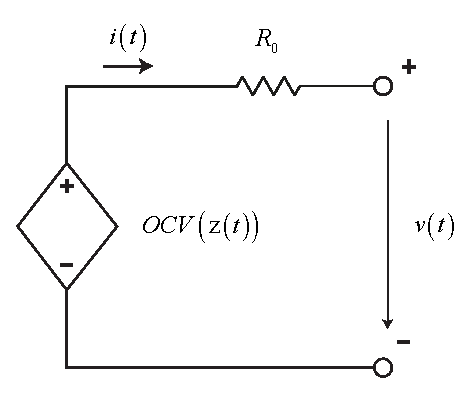
\includegraphics[width = 0.5\textwidth, width = 200pt, keepaspectratio]{figures/lithium_ion_battery/cell_eq_circuit_2.eps}
		\captionsetup{width=0.75\textwidth}		
		\caption{Improved cell model, with SOC-dependent voltage and equivalent series resistance $R_0$.}
		\label{ocv_soc_3}
	\end{subfigure}
	\caption{Equivalent circuit of the cell.}
	\label{}
\end{figure}
Experimentally we can observer that when the cell is subjected to a load (discharging) the terminal voltage drops below the open-circuit voltage and the terminal voltage rises above the open-circuit voltage when the cell is being charged. This phenomenon can be explained, in part, by placing a resistance in series with the controlled voltage source. The revised model is drawn in Figure~\ref{ocv_soc_3}. The added circuit component represent the so-called \textit{equivalent series resistance} (ESR) of the cell.

In the revised model, the state of the charge equation remains unchanged. However, we add a second equation to the model to describe how to compute the terminal voltage. In continuous time, we have
\begin{equation}
	\left\lbrace \begin{aligned}
		&\frac{dz(t)}{dt} = -\frac{1}{Q}\eta(t)i(t) \\[6pt]
		&v(t) = OCV(z(t)) - i(t)R_0
	\end{aligned}\right. 
\end{equation}
with this model, we see that $v(t)>OCV(z(t))$ when $i(t)<0$ (i.e. when charging) and $v(t)<OCV(z(t))$ when $i(t)>0$ (i.e. when discharging). 

Finally, we note that the cell's resistance is often a function of the cell's state of charge and is always a function of the cell's internal temperature. The fidelity of the model's predictions will be enhanced if these dependencies are taken into account in $R_0$.

\textbf{Polarization} refers to any deviation of the cell's terminal voltage away from open-circuit voltage due to a passage of current through the cell. In the equivalent circuit model we have modeled instantaneous polarization via the $i(t)R_0$ term. Real cells have more complex behaviour, where the voltage polarization slowly develops over time as current is demanded from the cell and then slowly decay over time when the cell is allowed to rest.

\begin{minipage}{0.4\textwidth}% adapt widths of minipages to your needs
	\includegraphics[width=\linewidth]{figures/lithium_ion_battery/cell_response_1.eps}
	\captionof{figure}{Behavior of the cell polarization, when a cell is subjected to a discharge pulse followed by a rest.}
	\label{polarization_1}
\end{minipage}%
\hfill%
\begin{minipage}{0.55\textwidth}
	Figure~\ref{polarization_1} illustrates this slower behaviour. The voltage plotted int the figure corresponds to the following scenario: \begin{enumerate}
		\item the cell is at the rest for the first 5 minute, and the voltage is constant
		\item the cell is then subjected to a discharge current pulse of constant magnitude from $t=\SI{5}{\minute}$ until $t=\SI{20}{\minute}$
		\item the load is removed and the cell is kept at rest for the remain of the test. 
	\end{enumerate}
The model we have developed up to now is not able to explain the dynamic behaviour presents in the test shown in Figure~\ref{polarization_1}.
\end{minipage}

The phenomenon shown in Figure~\ref{polarization_1} and which we witness every time we use a battery-powered device is mainly due to the slow diffusion process of lithium in  lithium-ion cell, so we will refer to this slowly changing in a circuit using one or more parallel resistor-capacitor sub-circuits. The equivalent circuit model become as follows
\begin{equation}
	\left\lbrace \begin{aligned}
		&	\frac{dz(t)}{dt} = -\frac{1}{Q}\eta(t)i(t) \\[6pt]
		&	\frac{di_{R_1}(t)}{dt} = -\frac{1}{R_1C_1}\Big(i_{R_1}(t)-i(t)\Big) \\[6pt]
		&	v(t) = OCV(z(t)) - i_{R_1}(t)R_1 - i(t)R_0
	\end{aligned}\right. 
\end{equation}
where its representation in discrete time domain becomes as follows
\begin{equation}
	\left\lbrace \begin{aligned}
		&	z[k+1] =z[k] -\frac{t_s}{Q}\eta[k]i[k] \\[6pt]
		&	i_{R_1}[k+1] = \exp\Big(-\frac{t_s}{R_1C_1}\Big)i_{R_1}[k]+\Big[1-\exp\Big(-\frac{t_s}{R_1C_1}\Big)\Big]i[k] \\[6pt]
		&	v[k] = OCV\Big(z[k]\Big) -R_1i_{R_1}[k] - R_0i[k]
	\end{aligned}\right. 
\end{equation}
\begin{figure}[H]
	\centering
	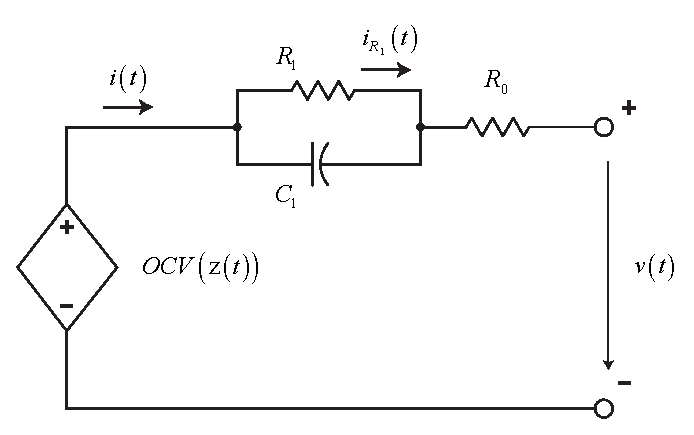
\includegraphics[width = 0.5\textwidth, width = 275pt, angle = 0, keepaspectratio]{figures/lithium_ion_battery/cell_eq_circuit_3.eps}
	\captionsetup{width=0.5\textwidth}		
	\caption{Circuit that models the diffusion voltage process.}
	\label{ocv_soc_4}
\end{figure}
Finally, we note that a cell's diffusion-voltage response is generally a function of the cell's state of charge and its internal temperature. If $R_1$ and $C_1$ are modeled as function of $z(t)$ and $T(t)$, the model prediction can be improved.
\begin{figure}[H]
	\centering
	\includegraphics[width = 0.5\textwidth, width = 300pt, angle = 0, keepaspectratio]{figures/lithium_ion_battery/cell_response_2.eps}
	\captionsetup{width=0.5\textwidth}		
	\caption{Measuring parameter values from a pulse response.}
	\label{polarization_2}
\end{figure}
Now we are going to discuss about hysteresis behaviour if the cell. Considering a given $OCV$ as function of the $SOC$, it can be observed that if we discharge a cell to $50\%\ SOC$ and allow the cell to rest, the equilibrium voltage is lower than $OCV$. If we charge a cell to $50\%\ SOC$ and allow the cell to rest, the equilibrium voltage is higher than $OCV$. These observations indicate that there is hysteresis in the cell terminal voltage.

Let $h(z,t)$ be the dynamic hysteresis voltage as a function of $SOC$ and time. We model the change in hysteresis voltage as a function of change in $SOC$ as follows
\begin{equation}
	\frac{dh(z,t)}{dt} = \gamma\sign(\dot{z})\Big[M(z,\dot{z})-h(z,t)\Big]
\end{equation}
where $M(z,\dot{z})$ is a function that gives the maximum polarization due to hysteresis as a function of $SOC$ and the rate of charge od $SOC$.
Specifically, we require that $M(z,\dot{z})$ be positive for charge ($\dot{z}>0$) and negative for discharge ($\dot{z}<0$). The $M(z,\dot{z})-h(z,t)$ term is the differential equation states that the rate of charge of hysteresis voltage is proportional to the distance of the present hysteresis value away from the major hysteresis loop, leading to a kind of exponential decay of voltage to the major loop. The term in from of this has a positive constant $\gamma$ which tunes the rate of decay and $\sign(\dot{z})$, which forces the equation to be stable both for charge and discharge.

To fit the differential equation for $h(z,t)$ into out model, we must manipulate it to be a differential equation with respect to time, not with respect to $SOC$. We accomplish this by multiplying both side of the equation by $dz/dt$
\begin{equation}
	\frac{dh(z,t)}{dz}\frac{dz}{dt}=\gamma\sign(\dot{z})\Big[M(z,\dot{z})-h(z,t)\Big]\frac{dz}{dt}
\end{equation} 
we use the chain rule to write the left-hand side of the equation as $dh(z,t)/dt$ and we substitute $dz/dt = -\eta(t)i(t)/Q$ into the right hand side, noting that $\dot{z}\sign(\dot{z})=\abs{\dot{z}}$. Thus,
\begin{equation}
	\frac{dh(t)}{dt} = -\abs{\frac{\eta(t)i(t)\gamma}{Q}}h(t)+\abs{\frac{\eta(t)i(t)\gamma}{Q}}M(z,\dot{z}).
\end{equation}
This may be converted into a difference equation for out discrete-time application assuming $i(t)$ and $M(z,\dot{z})$ are constant over the sample period. 
\begin{equation}
h[k+1] = \exp\Bigg(-\abs{\frac{\eta[k]i[k]\gamma t_s}{Q}}\Bigg)h[k] + \Bigg[1-\exp\Bigg(-\abs{\frac{\eta[k]i[k]\gamma t_s}{Q}}\Bigg)\Bigg]M(z,\dot{z}).
\end{equation}
Note that this is a nonlinear time-varying system as the factors multiplying the state and input change with $i[k]$.
The simplest representation is when $M(z,\dot{z})=-M\sign(i[k])$, when 
 \begin{equation}
 	h[k+1] = \exp\Bigg(-\abs{\frac{\eta[k]i[k]\gamma t_s}{Q}}\Bigg)h[k] - \Bigg[1-\exp\Bigg(-\abs{\frac{\eta[k]i[k]\gamma t_s}{Q}}\Bigg)\Bigg]M\sign(i[k]).
 \end{equation}
With this representation $-M\le h[k] \le M$ at all times, and $h[k]$ has units of volts. When attempting to find the model parameters, we will find it valuable to rewrite this in an equivalent but slightly different representation, which has unitless hysteresis state $-1 \le h[k] \le 1$,
 \begin{equation}
	h[k+1] = \exp\Bigg(-\abs{\frac{\eta[k]i[k]\gamma t_s}{Q}}\Bigg)h[k] - \Bigg[1-\exp\Bigg(-\abs{\frac{\eta[k]i[k]\gamma t_s}{Q}}\Bigg)\Bigg]\sign(i[k]).
\end{equation}
\begin{equation}
\text{Hysteresis voltage } = Mh[k].
\end{equation}


This makes the output equation linear in $M$.

In additional to the type of dynamic hysteresis that changes as $SOC$ changes, we also can modeling an instantaneous change in hysteresis voltage when the sign of the current changes.
\begin{equation}
	s[k]=\left\lbrace \begin{aligned}
		&\sign(i[k]) \qquad\abs{i[k]>0} \\[6pt]
		&s[k-1], \qquad\text{otherwise}
	\end{aligned}\right. 
\end{equation}
Then the instantaneous hysteresis is modeled as
\begin{equation}
	\text{Instantaneous hysteresis voltage } = M_0s[k].
\end{equation}
and overall hysteresis is
\begin{equation}
	\text{Hysteresis voltage } = M_0s[k] + Mh[k].
\end{equation}

\begin{mybox}
	\textbf{Enhanced self-correcting (ESC) model state equations}
\begin{equation}\label{lithium_ion_battery_model}
	\left\lbrace \begin{aligned}
		&	z[k+1] =z[k] -\frac{t_s}{Q}\eta[k]i[k] \\[6pt]
		&	i_{R_1}[k+1] = \exp\Big(-\frac{t_s}{R_1C_1}\Big)i_{R_1}[k]+\Big[1-\exp\Big(-\frac{t_s}{R_1C_1}\Big)\Big]i[k] \\[6pt]
		&	h[k+1] = \exp\Bigg(-\abs{\frac{\eta[k]i[k]\gamma t_s}{Q}}\Bigg)h[k] - \Bigg[1-\exp\Bigg(-\abs{\frac{\eta[k]i[k]\gamma t_s}{Q}}\Bigg)\Bigg]\sign(i[k]) \\[6pt]
		&	s[k]= \left\lbrace 
			\begin{aligned}
				& \sign(i[k]) \qquad\abs{i[k]>0} \\[6pt]
				& s[k-1], \qquad\text{otherwise}
			\end{aligned}\right.  \\[6pt]
		&	v[k] = OCV\Big(z[k],T[k]\Big)+ M_0 s[k] + M h[k] -R_1i_{R_1}[k] - R_0i[k]
	\end{aligned}\right. 
\end{equation}

\begin{figure}[H]
	\centering
	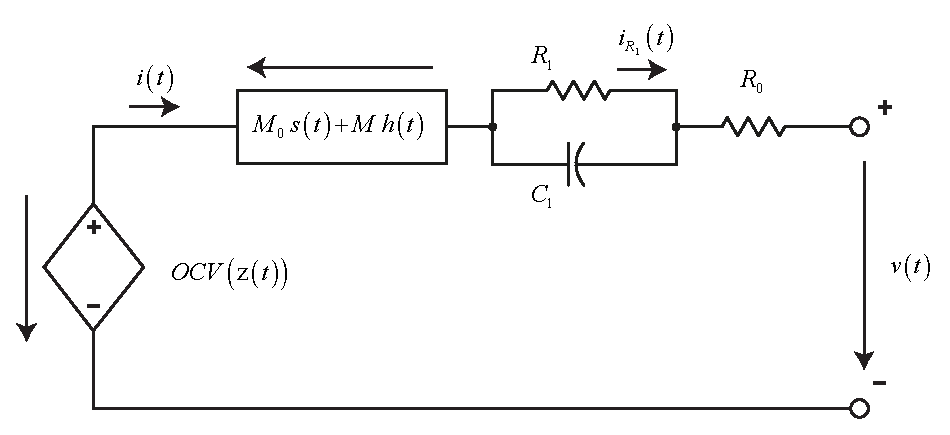
\includegraphics[width = 0.5\textwidth, width = 360pt, angle = 0, keepaspectratio]{figures/lithium_ion_battery/cell_eq_circuit_4.eps}
	\captionsetup{width=0.5\textwidth}		
	\caption{The enhanced self-correcting cell model equivalent circuit.}
	\label{ocv_soc_5}
\end{figure}
\end{mybox}

\section{Open circuit voltage model}
To find an analytical model of the open circuit voltage of the lithium ion cell plays a fundamental role in the development of a battery management system. The open circuit voltage of a lithium ion cell is a quantity which can be measured with very high accuracy and the knowledge of the model (and its matching) permits to determine the state of charge of the battery.

The model of the $OCV(z)$ as function of the $z=SOC(t)$ can be represented as follows
\begin{equation}
 	\begin{aligned}
		OCV(z) = E_{-1}\exp(-z\alpha) + E_0 + E_1z + E_2z^2 + E_3z^3 +  E_\text{log}\log({1-z})
	\end{aligned}
\end{equation}
where $z$ belong to an open set as $z\in\left(0\ 1\right)$.

For the sake of clarity we can consider the following case:
\begin{itemize}
	\item[$-$] $E_{-1}=\SI{-1.031}{\volt}$
	\item[$-$] $\alpha=\SI{35}{}$
	\item[$-$] $E_0=\SI{3.685}{\volt}$
	\item[$-$] $E_1=\SI{0.015}{\volt}$
	\item[$-$] $E_2=\SI{0}{\volt}$
	\item[$-$] $E_3=\SI{0}{\volt}$
	\item[$-$] $E_\text{log}=\SI{-0.05}{\volt}$
\end{itemize}
which results in a $OCV(z)$ curve as shown in Figure~\ref{ocv} 
\begin{figure}[H]
	\centering
	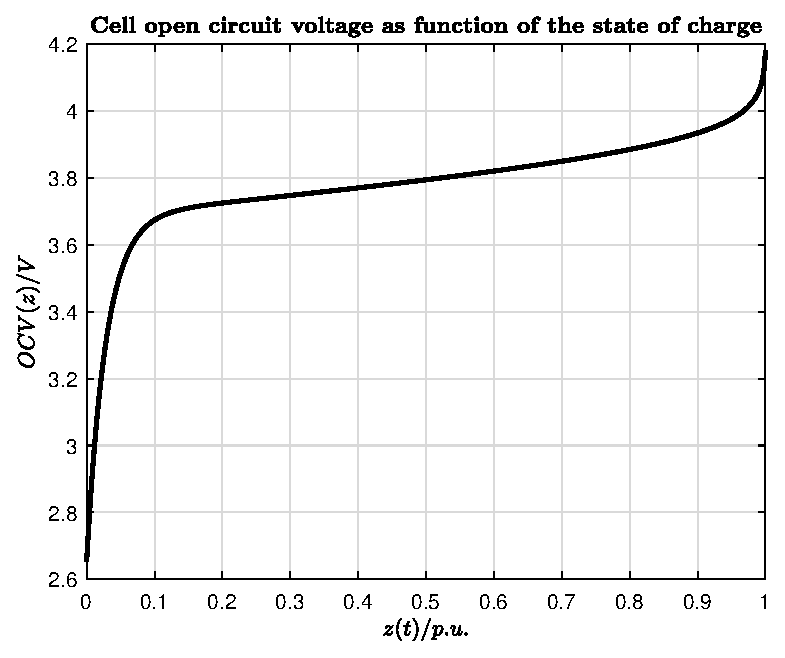
\includegraphics[width = 0.5\textwidth, width = 300pt, angle = 0, keepaspectratio]{figures/lithium_ion_battery/ocv.eps}
	\captionsetup{width=0.5\textwidth}		
	\caption{Lithium-ion battery open circuit cell as function of the state of charge.}
	\label{ocv}
\end{figure}

\section{Model parameters settings}
Parameters of the model are based on equations \eqref{lithium_ion_battery_model} and by the equivalent electrical model shown in Figure~\ref{ocv_soc_5}. Model equations cab be split into two parts: first part describe transport and electrochemical equation. The second part refers to the equivalent electrical model where additional voltage drop are accounted. 
\begin{itemize}
	\item[$-$] \textbf{Charge Capacity} $Q[\SI{}{\ampere\hour}]$: is the nominal charge capacity of the battery.
	\item[$-$] \textbf{Number of Cells} $N_\text{cell}[\SI{}{}]$: is the number of internal lithium ion cells.
	\item[$-$] \textbf{Open Circuit Voltage Model} 
	\begin{itemize}
		\item[$-$] $E_{-1}\ [\SI{}{\volt}]$
		\item[$-$] $\alpha\ [p.u.]$
		\item[$-$] $E_{0}\ [\SI{}{\volt}]$
		\item[$-$] $E_{1}\ [\SI{}{\volt}]$
		\item[$-$] $E_{2}\ [\SI{}{\volt}]$
		\item[$-$] $E_{3}\ [\SI{}{\volt}]$
		\item[$-$] $E_{log}\ [\SI{}{\volt}]$
	\end{itemize}
	\item[$-$] $R_{0}\ [\SI{}{\ohm}]$: internal resistance $R_0$
	\item[$-$] $R_{1}\ [\SI{}{\ohm}]$: internal resistance $R_1$
	\item[$-$] $C_{1}\ [\SI{}{\farad}]$: double layer membrane capacity
	\item[$-$] $M\ [\SI{}{\volt}]$: hysteresis parameter
\end{itemize}

\section{Model output variables}
The output bus channel \textbf{Lithium-Ion-Battery data} includes the following data output
\begin{itemize}
	\item[$-$] $i_\text{out}$: battery output current in $\Big[\SI{}{\ampere}\Big]$.
	\item[$-$] $v_\text{out}$: battery output voltage in $\Big[\SI{}{\volt}\Big]$.  
	\item[$-$] $SOC$: state of charge in $[p.u.]$
	\item[$-$] $i_\text{in}$: battery input current in $\Big[\SI{}{\ampere}\Big]$.
\end{itemize}
\begin{thebibliography}{99}

	\bibitem[\textbf{G. Plett, 2015}]{p14} Gregory L. Plett - \textit{Battery Modeling. Volume I}. Artech House 2015.
	
	\bibitem[\textbf{G. Plett, 2015}]{p15} Gregory L. Plett - \textit{Battery Modeling. Volume II}. Artech House 2015.
	
	\bibitem[\textbf{G. Plett, 2004}]{p16} Gregory L. Plett - \textit{Extended Kalman filtering for battery management systems of LiPB/based HEV battery packs. Part 1. Background}. Journal of Power Sources 134 (2004).
	
	\bibitem[\textbf{G. Plett, 2004}]{p17} Gregory L. Plett - \textit{Extended Kalman filtering for battery management systems of LiPB/based HEV battery packs. Part 2. Modeling and identification}. Journal of Power Sources 134 (2004).	
	
	\bibitem[\textbf{G. Plett, 2004}]{p18} Gregory L. Plett - \textit{Extended Kalman filtering for battery management systems of LiPB/based HEV battery packs. Part 3. State and parameter estimation}. Journal of Power Sources 134 (2004)
	
\end{thebibliography}
\end{document} 